\IfFileExists{ajr.sty}
{\documentclass[12pt]{article}\usepackage[a5paper,margin=5mm]{geometry}}
{\documentclass[12pt,a4paper]{article}}



\usepackage{url,natbib}
\let\harvardurl\url
\usepackage{graphicx,amsmath,amsfonts,defns}
\allowdisplaybreaks
\usepackage{pgfplots}
\usepgfplotslibrary{external} %exports pdf for each tikz figure
\tikzexternalize
%\tikzset{external/force remake}%forces redraw of all tikz graphics

\usepackage{pdfcomment}
\newcommand{\ajr}[1]{\pdfcomment[author=AJR,color={0.8 0.8 0},subject={#1}]{#1}}


%\numberwithin{equation}{section}
%\numberwithin{figure}{section}
%\numberwithin{table}{section}

\newcommand{\bc}{\textsc{bc}}
\newcommand{\cc}{\textsc{cc}}

\def\ajrSplit#1#2\ajrEndSplit{\def\ajrcar{#1}\def\ajrcdr{#2}}
\def\Vec{}
\renewcommand{\Vec}[1]{%
  \typeout{**** Command  \ #1v denotes vector #1}%
  \expandafter\ajrSplit#1\ajrEndSplit%
  \ifx\ajrcdr\empty % single character
    \expandafter\def\csname#1v\endcsname%
    {\ensuremath{\vec #1}}%
  \else % multicharacter e.g. greek
    \expandafter\def\csname#1v\endcsname%
    {\ensuremath{\vec{\csname#1\endcsname}}}%
  \fi%
  }
\Vec U \Vec g \Vec v \Vec u \Vec s

\newcommand{\Bb}[1]{%
  \expandafter\def\csname#1#1\endcsname%
  {\ensuremath{\mathbb #1}}}
\Bb X\Bb T\Bb R\Bb I\Bb J \Bb E

\newcommand{\Cal}[1]{%
  \expandafter\def\csname c#1\endcsname%
  {\ensuremath{\mathcal #1}}}
\Cal L \Cal I \Cal N \Cal M

\newcommand{\secref}[1]{\ref{sec:#1}}

\title{An exciting application of piecewise-linear holistic discretisation}
\author{G.~A. Jarrad 
\and 
A.~J. Roberts\thanks{School of Mathematical Sciences, University of Adelaide, South Australia~5005, Australia.  
\protect\url{mailto:anthony.roberts@adelaide.edu.au}}
}
\begin{document}
\maketitle

\begin{abstract}
\ajr{Need to shorten}
The fidelity of numerical simulation of a spatio-temporal dynamical system is 
largely constrained by the chosen discretisation of the \pde{}. 
In particular, the modeller is typically free to choose
arbitrary finite-element forms for the various spatial derivatives,
without necessarily having knowledge of the accuracy of the resulting numerical schemes.
The holistic discretisation approach described in this paper obviates the problem of arbitration. % mediation?

Centre manifold theory is applied to derive an asymptotically accurate
representation of the microscale dynamics of the one-dimensional Burgers' equation. 
In the process, the corresponding macroscale dynamics 
are constrained to match the microscale solution at discrete grid-points.
The resulting representation of macroscale evolution provides an unambiguous discretisation of the \pde{},
suitable for numerical simulation. 

The iterative process starts with a choice of the leading, macroscale approximation to the linearised system.
Suitable internal boundary conditions are then induced on the spatial derivatives 
at the end-points of each discrete interval.
Although the choice of IBCs might appear to be arbitrary, they are in fact governed by the placement of the grid-points and the 
form of the leading discrete approximation.
The particular approach taken here is to start with a piecewise linear but continuous approximation,
in contrast to similar analyses that use piecewise constant, discontinuous approximations.
This is motivated by the principle that a more accurate leading approximation should lead to faster
convergence of the asymptotic solution, via the Rayleigh-Ritz theorem.

Further iterations of the centre manifold process lead inexorably to a temporal evolution formulation of the macroscale dynamics,
holistically informed by the underlying microscale dynamics.  
We examine the accuracy and stability of the resulting numerical scheme, in comparison to
the behaviours of several other typical approximations.
\end{abstract}






\section{Introduction}\label{sec:intro}

This article's scope is the accurate spatial discretisation of nonlinear \pde{}s for a field~\(u(x,t)\) satisfying reaction-advection-diffusion \pde{}s in the general form
\begin{equation}
u_t=F(u_x)_x+\alpha G(x,u,u_x)
\label{eq:genpde}
\end{equation}
where subscript \(x\) and~\(t\) denote derivatives, and for smooth functions \(F\) and~\(G\).
Given \(N\)~discrete points in space, \(x=X_j\) for \(j=1,\ldots,N\)\,, we define grid values \(U_j(t)=u(X_j,t)\)\,.
Then the aims are to: firstly, establish that in principle there exists an \emph{exact} closure of the dynamics of the \pde~\eqref{eq:genpde} in terms of these grid values, \(d\\Uv/dt=\gv(\Uv)\); secondly,  establish that such a closure is emergent from general initial conditions; thirdly, show how to construct systematic approximations to the in-principle closure; and fourthly, evaluate its performance for the classic example of the nonlinear advection--diffusion Burgers' \pde
\begin{eqnarray}
	\D tu = \nu\DD xu - \alpha u\D xu\,.
\label{eq:burgers}
\end{eqnarray}
Generalisation of the approach to two or more spatial dimensions remain for further research.

%Mention cole-hopf leads to known solution which is unconditionally stable.
The spatial domain~\(\XX\) is of length~\(L\), \(0\leq x\leq L\)\,, and we mostly restrict attention to solutions~\(u(x,t)\) which are \(L\)-periodic in space, but occasionally comment on the cases of Dirichlet boundary conditions, \(u(0,t)=u(L,t)=0\)\,, and Neumann boundary conditions, \(u_x(0,t)=u_x(L,t)=0\)\,.
The first step is to partition~$\XX$ into $N$~equi-spaced intervals bounded by $N+1$~grid-points~\(X_j\), \({j=0,\ldots,N}\), with spacing~\(H\).
Traditional spatial discretisation of such \pde{}s, whether finite difference, finite element, or finite volume, imposes assumed fields in each element and then derives approximate rules for the evolution in time of the parameters of the imposed fit.

Our approach is to let the \pde~\eqref{eq:burgers} determine the subgrid structures in order to remain faithful to the \pde.
Let the dynamics of the field~$u(x,t)$ be summarised by the coarse dynamics ${\Uv}=(U_1,U_2,\ldots,U_N)$, where grid values \begin{equation}
U_j(t):=u(X_j,t)\text{ for all }t\in \TT.
\label{eq:gridval}
\end{equation}
Theory to be discussed asserts that in principle and \emph{exact} closure exists: that is, there is some coarse temporal evolution 
\begin{eqnarray}
	\dot{\Uv}(t) = {\gv}({\Uv})
\label{eq:temporal}
\end{eqnarray}
that gives exact solutions of the \pde.
The traditional approach is to use centred approximations, for two examples,  
\begin{eqnarray*}
\DD xu&\approx& \frac1{H^2}(U_{j+1}-2U_j+U_{j-1})=\delta^2 U_j/H^2;
\\
u\D xu&\approx&\frac1{2H}U_j(U_{j+1}-U_{j-1})=U_j\mu\delta U_j/H\,;
\end{eqnarray*}
where the centred difference $\delta=\sigma^{1/2}-\sigma^{-1/2}$,
centred mean $\mu=(\sigma^{1/2}+\sigma^{-1/2})/2$,
and the shift operator $\sigma U_j=U_{j+1}$.
However, the nonlinear advection term has another plausible representation, namely the conservative form~$\mu\delta (U_j^2)/2H$.
For illustrative purposes, a convex combination of the two  representations will be used for comparison; that is, we will compare results with Burgers' \pde~\eqref{eq:burgers} discretised to
\begin{eqnarray}
	\dot{U}_j = \nu\frac{\delta^2 U_j}{H^2}
	-(1-\theta)\alpha\frac{U_j\mu\delta U_j}{H}
    -\theta\alpha\frac{\mu\delta (U_j^2)}{2H}\,.
\label{eq:mixture}
\end{eqnarray}
In contrast, Section~\secref{nonlin} shows our holistic approach has no such representational ambiguity, and constructs at first-order the specific model
\begin{eqnarray}
	\dot{U}_j = S\left[\nu\frac{\delta^2 U_j}{H^2}
	-\alpha\frac{U_j\mu\delta U_j}{3H}
    -\alpha\frac{\mu\delta (U_j^2)}{3H}\right],
\label{eq:holistic1}
\end{eqnarray}
where the nonlocal operator $S=(1+\delta^2/6)^{-1}$. 
Observe that, apart from the nonlocal operator~$S$,
this holistic model matches the mixture model~\eqref{eq:mixture} for parameter $\theta=\frac{2}{3}$.
This parameter value is exactly the critical value predicted by \cite{Fornberg73} to be necessary for stable simulation (with $\nu=0$ and $\alpha=1$) for a selection of numerical integration schemes.
Section~\secref{numeric} further compares the numerical behaviour of the holistic and mixture models.

The final part of the process is to express the physical field~\(u(x,t)\) in terms of the coarse solution~${\Uv}(t)$. 
That is, we construct the field
\begin{eqnarray}
	u  = {u}(x,{\Uv}),
	\label{eq:spatial}
\end{eqnarray}
where the time evolution of~\(u\) comes via the evolving coarse variable~\(\Uv\).
The complete holistic framework comprises equations~\eqref{eq:temporal} and \eqref{eq:spatial},  along with the addition of suitable boundary conditions that are discussed in Section~\secref{lin}.
Section~\secref{nonlin} shows that, to first-order, the holistic mapping $\hat{u}$ takes the form
\begin{eqnarray}
\hat{u} = \sum_{j=1}^{N}\chi_j\left({\cI}_{0}U_j+\frac{H^2}{6\nu}{\cI}_{1}\dot{U}_j
+\frac{\alpha H}{6\nu}{\cI}_{1}U_j\,\Delta U_j\right)\,,
\end{eqnarray}
with backward-difference $\nabla=1-\sigma^{-1}$ and interpolators ${\cI}_{0}=\sigma^{-1}+\xi\nabla$ and
${\cI}_{1}=\xi^3+(1-\xi)^{3}\sigma^{-1}-\xi\nabla-\sigma^{-1}$,
using the interval indicator $\chi_j(x)=1$ (else $0$) for $X_{j-1}\le x<X_j$ and
dimensionless coordinate $\xi(x)=\sum_{j=1}^{N}\chi_j(x)\frac{x-X_{j-1}}{H}$.
Figure~\ref{fig:uhat} shows an example of the holistic approximation $\hat{u}(x,t)$ to the true field $u(x,t)$.
\begin{figure}
\centering
\tikzsetnextfilename{smoothInterp}
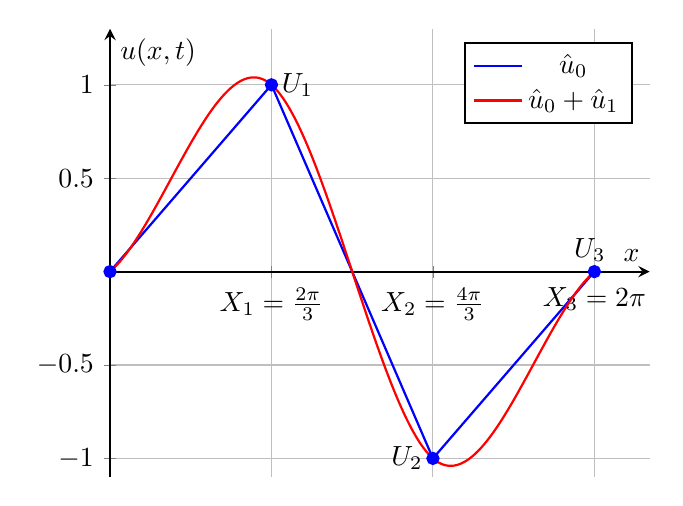
\begin{tikzpicture}[declare function = { 
	xi1(\x) = \x/2.0944; xi2(\x) = \x/2.0944-1; xi3(\x) = \x/2.0944-2; 
	u0(\x) = 0; u1(\x) = 1; u2(\x) = -1; u3(\x) = 0;
	sd2u0(\x) = -4.5*u0(\x)+3*u1(\x)-1.5*u2(\x)+3*u3(\x);
	sd2u1(\x) = -4.5*u1(\x)+3*u2(\x)-1.5*u3(\x)+3*u0(\x);
	sd2u2(\x) = -4.5*u2(\x)+3*u3(\x)-1.5*u0(\x)+3*u1(\x);
	sd2u3(\x) = -4.5*u3(\x)+3*u0(\x)-1.5*u1(\x)+3*u2(\x);
}]
\begin{axis}[ xlabel={$x$}, ylabel={$u(x,t)$}
  ,axis x line=middle,axis y line=middle
  ,thick,grid,samples=101
  ,ymin=-1.1,ymax=1.3 ,domain=0:6.2832,xmax=7
  ,xtick={2.0944,4.1888,6.2832}
  ,xticklabels={$X_1=\frac{2\pi}{3}$,$X_2=\frac{4\pi}{3}$,$X_3=2\pi$}
  ,legend pos=north east
  ] 
\addplot [blue,no marks,domain=0:2.0944] {xi1(x)*u1(x)+(1-xi1(x))*u0(x)}; 
\addlegendentry{$\hat{u}_0$};
\addplot [red,no marks,domain=0:2.0944] {xi1(x)*u1(x)+(1-xi1(x))*u0(x)
	+1/6*(xi1(x)^3*sd2u1(x)+(1-xi1(x))^3*sd2u0(x)-xi1(x)*(sd2u1(x)-sd2u0(x))-sd2u0(x))
}; 
\addlegendentry{$\hat{u}_0+\hat{u}_1$};
\addplot [blue,no marks,domain=2.0944:4.1888] {xi2(x)*u2(x)+(1-xi2(x))*u1(x)}; 
\addplot [blue,no marks,domain=4.1888:6.2832] {xi3(x)*u3(x)+(1-xi3(x))*u2(x)}; 
\addplot [red,no marks,domain=2.0944:4.1888] {xi2(x)*u2(x)+(1-xi2(x))*u1(x)
	+1/6*(xi2(x)^3*sd2u2(x)+(1-xi2(x))^3*sd2u1(x)-xi2(x)*(sd2u2(x)-sd2u1(x))-sd2u1(x))
}; 
\addplot [red,no marks,domain=4.1888:6.2832] {xi3(x)*u3(x)+(1-xi3(x))*u2(x)
	+1/6*(xi3(x)^3*sd2u3(x)+(1-xi3(x))^3*sd2u2(x)-xi3(x)*(sd2u3(x)-sd2u2(x))-sd2u2(x))
}; 
\addplot [blue,only marks,mark=*] coordinates 
{(0,0)(2.0944,1)(4.1888,-1)(6.2832,0)};
\node[right] at (axis cs:2.0944,1) {$U_1$};
\node[left] at (axis cs: 4.1888,-1) {$U_2$};
\node[above] at (axis cs: 6.2832,0) {$U_3\ $};
\end{axis}
\end{tikzpicture}
\caption{An example of the smooth subgrid field provided by the holistic discretisation process,
where the piecewise-linear initial approximation~$\hat{u}_0$ is smoothed by the first-order correction~$\hat{u}_1$  (for nonlinearity $\alpha=0$).
The correction takes the form of a cubic spline; however, it is derived directly from the \pde\ itself, rather than obtained by 
imposing an interpolation.}
\label{fig:uhat}
\end{figure}





\section{A basic example introduces theory and method}
\label{sec:beitm}

This section investigates the modelling of Burgers' \pde~\eqref{eq:burgers} on the specific domain \(-1<x<1\)\,, with basic Dirichlet boundary conditions that \(u(\pm 1,t)=0\)\,, and with viscosity \(\nu=1\) for definiteness.
For introductory simplicity, the domain space is partitioned into just two intervals, \(-1<x<0\) and \(0<x<1\)\,, by a `grid point' \(X=0\)\,.
Our aim is to model the dynamics of the whole field~\(u(x,t)\) by simply the dynamics of the `grid value' \(U(t):=u(0,t)\) of the field at this central grid point.

The dynamics in the two intervals need to be coupled to each other to form a solution valid over the whole domain.
Conventional numerical methods \emph{impose} an assumed interpolation field and then derive a corresponding model.
In contrast, here we craft a coupling that moderates the communication between the two intervals, and then left the \pde~\eqref{eq:burgers} itself tell us the appropriate fields and model.
The desired full coupling between the two intervals is of \(C^1\)~continuity: \([u]=[u_x]=0\) where we introduce~\([\cdot]\) to denote the jump in value across the grid point \(X=0\)\,, that is, \([u]=u|_{0^+}-u|_{0^-}\)\,.
For reasons developed below, we embed Burgers' \pde~\eqref{eq:burgers} in a family of problems with the moderated coupling between intervals of
\begin{equation}
[u]=0\quad\text{and}\quad
[u_x]+2(1-\gamma)u=0 \quad\text{at }x=0\,;
\label{eq:cc1}
\end{equation}
that is, the field is continuous but the derivative has a discontinuity depending upon parameter~\(\gamma\).  
We derive below that parameter \(\gamma=0\) provides a useful base to apply powerful centre manifold theory.
When parameter \(\gamma=1\) the coupling~\eqref{eq:cc1} reverts to requiring \(C^1\)~continuity across \(x=0\) to restore the \pde.

To show there is a useful centre manifold, we start with equilibria in the system.
The diffusion \pde~\eqref{eq:burgers}, with nonlinearity \(\alpha=0\) and diffusivity \(\nu=1\), together with coupling conditions~\eqref{eq:cc1}, and the Dirichlet boundary conditions, has a subspace~\EE\ of equilibria: for each~\(U\),
\begin{equation}
u=(1-|x|)U\quad\text{and }\gamma=0\,.
\label{eq:equil}
\end{equation}
The spectrum about these equilibria determine the manifold structure.
Seek linearised solutions \(u\approx (1-|x|)U+e^{\lambda t}v(x)\) for small~\(v\):  the diffusion \pde~\eqref{eq:burgers} becomes the eigenproblem
\begin{equation}
-v_{xx}+\lambda v=0\,,
\quad\text{such that }[v]=[v_x]+2v=0\text{ at }x=0\,,
\label{eq:lindiff}
\end{equation}
and the homogeneous Dirichlet boundary conditions \(v(\pm 1)=0\)\,.
\begin{itemize}
\item Corresponding to eigenvalue \(\lambda=0\) is the neutral solution \(v\propto1-|x|\) reflecting the direction of the subspace of equilibria.
\begin{figure}
\centering
\begin{tabular}{cc}
\tikzsetnextfilename{simpevec}
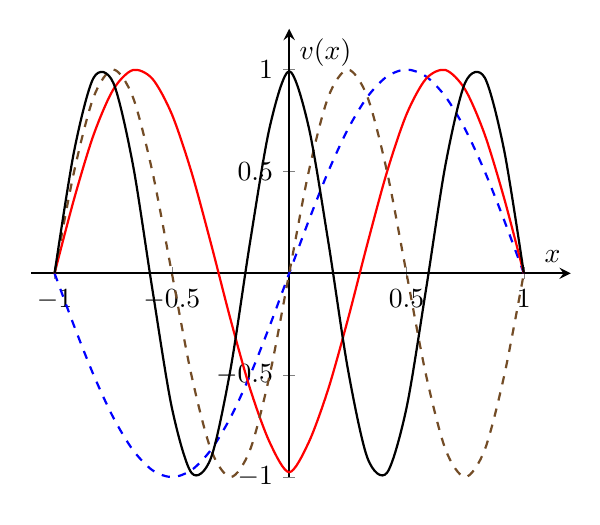
\begin{tikzpicture}
\begin{axis}[xlabel={$x$},ylabel={$v(x)$}
,domain=-1:1,axis x line=middle, axis y line=middle
,ymax=1.2,xmin=-1.1,xmax=1.2,thick,smooth]
    \addplot+[dashed,no marks] {sin(180*x)};
    \addplot+[no marks] {sin(4.4934*180/3.1416*(1-abs(x))};
    \addplot+[dashed,no marks] {sin(360*x)};
    \addplot+[no marks] {sin(7.7253*180/3.1416*(1-abs(x))};
\end{axis}
\end{tikzpicture}
&
\parbox[b]{0.45\linewidth}{\caption{\label{fig:simpevec}\sloppy%
eigenfunctions~\(v(x)\) of the linearised problem~\eqref{eq:lindiff} corresponding to negative eigenvalues: blue dashed,~\(-\pi^2\); red solid,~\(-20.191\); brown dashed,~\(-4\pi^2\); and black solid,~\(-59.680\).}}
\end{tabular}
\end{figure}

\item Negative eigenvalues \(\lambda=-k^2\) arise corresponding to eigenfunctions of the form \(v\propto\sin[k(1-|x|)]\) by necessity from the \pde, the homogeneous Dirichlet boundary conditions, and the continuity of~\(v\).
By straightforward algebra, the jump in the derivative determines the wavenumbers from the solutions of \(k=\tan k\)\,, namely the wavenumbers \(k=4.4934,7.7253,10.9041,\ldots\)\,.
That is,  non-zero eigenvalues of the linearised problem are \(\lambda=-20.191,-59.680,-118.900,\ldots\)\,.
Figure~\ref{fig:simpevec} plots (solid) the corresponding eigenfunctions for the two smallest magnitude of these eigenvalues.

\item Negative eigenvalues also arise from eigenfunctions of the form \(v\propto\sin(kx)\).  
The boundary and coupling conditions determine that wavenumbers \(k=n\pi\) for \(n=1,2,3,\ldots\)\,.
That is, the other non-zero eigenvalues are \(\lambda=-\pi^2, -4\pi^2, -9\pi^2, \ldots\)\,.
Figure~\ref{fig:simpevec} plots (dashed) the corresponding eigenfunctions for the two smallest magnitude of these eigenvalues.
\end{itemize}
One of the beautiful properties of the coupling conditions~\eqref{eq:cc1} is that with them the diffusion operator~\(\DD x{}\) is self-adjoint.
Hence there are only real eigenvalues of the linear problem~\eqref{eq:lindiff}, namely the ones found above.
To confirm self-adjointness under the usual inner product, \(\left<u,v\right>=\int_{-1}^1 u(x)v(x)\,dx\)\,,
consider
\begin{eqnarray*}
\left<u,v_{xx}\right>
&=&\int_{-1}^1 uv_{xx}\,dx
\quad(\text{then using integration by parts})
\\&=&\left[uv_{x}-vu_{x}\right]_{-1}^{0^-}
+\left[uv_{x}-vu_{x}\right]_{0^+}^1+\int_{-1}^1 u_{xx} v\,dx
\\&&\quad(\text{using the Dirichlet boundary conditions})
\\&=&-\left[uv_{x}-vu_{x}\right]_{0^-}^{0^+}+\left<u_{xx},v\right>
\\&&\quad(\text{using continuity at }x=0)
\\&=&-u|_0[v_{x}]+v|_0[u_{x}]+\left<u_{xx},v\right>
\\&&\quad(\text{using the jump in derivative at }x=0)
\\&=&u|_02(1-\gamma)v|_0-v|_02(1-\gamma)u|_0+\left<u_{xx},v\right>
\\&=&\left<u_{xx},v\right>.
\end{eqnarray*}
Hence it is self-adjoint.
This useful self-adjointness is not a property of previous holistic discretisations, but is a new feature maintained for the approach of this article.

Because the spectrum consists of a zero eigenvalue and all the rest negative (\(\leq -\pi^2<-9\)), centre manifold theory \cite[e.g.]{Carr81} 
%or \cite[Chap.~4]{Roberts2014a}
assures us that there exists a slow manifold in some neighbourhood of the subspace~\EE\ of equilibria: that is, global in amplitude~\(U\) and local in parameter~\(\gamma\).
Also, theory guarantees that all solutions in the neighbourhood are attracted exponentially quickly, roughly like~\(e^{-9t}\), to solutions on the slow manifold.
That is, the slow manifold and the evolution thereon emerges from general initial conditions.

Lastly, a theorem also guarantees that when we approximate the slow manifold and its evolution to a residual of~\Ord{\gamma^p}, the the slow manifold and its evolution are correct to errors~\Ord{\gamma^p}.
By straightforward machinations not detailed here~\cite[Ch.~14]{Roberts96a, Roberts2014a} we arrive at the expressions that the slow manifold and the evolution thereon are
% see tiwdbc.tex for Reduce code
\begin{equation}
u\approx\left[1-|x|+\gamma(|x|-\tfrac32x^2+\tfrac12|x|^3)\right]U
\quad\text{such that }\dot U\approx-3\gamma U\,.
\label{eq:egsm1}
\end{equation}
Substituting these expressions into the heat \pde~\eqref{eq:burgers} (\(\alpha=0\)), and the boundary and coupling conditions~\eqref{eq:cc1} we find the equations are satisfied to residual~\Ord{\gamma^2} and so the approximation theorem asserts these expressions are approximations with errors~\Ord{\gamma^2}.

\begin{figure}
\centering
\begin{tabular}{cc}
\tikzsetnextfilename{simpleshape}
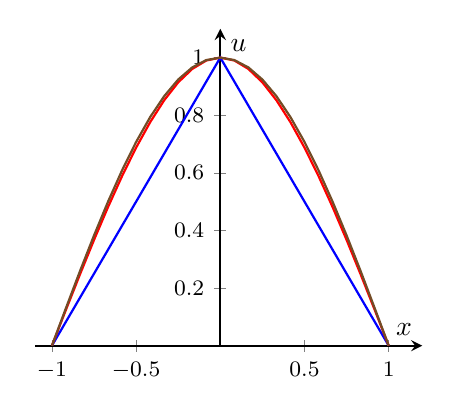
\begin{tikzpicture}
\begin{axis}[small,xlabel={$x$},ylabel={$u$}
,domain=-1:1,axis x line=middle, axis y line=middle
,ymax=1.1,xmin=-1.1,xmax=1.2,thick]
    \addplot+[no marks] {1-abs(x)};
    \addplot+[no marks] {1-1.5*x^2+abs(x)^3/2};
    \addplot+[no marks] {cos(90*x)};
\end{axis}
\end{tikzpicture}
&
\parbox[b]{0.55\linewidth}{\caption{\label{fig:simp}%
compare approximations to the long-term, quasi-stationary, decay of the heat \pde: blue, \(u\propto 1-|x|\) is the basic linear approximation~\eqref{eq:equil}; red, the derived cubic spline~\eqref{eq:egsm1} at full coupling \(\gamma=1\); and, almost indistinguishable, brown, is the exact mode \(u\propto\cos(\pi x/2)\).
}}
\end{tabular}
\end{figure}

Although this approximation is based around parameter \(\gamma=0\)\,, we are interested in the physical value of the parameter \(\gamma=1\)\,.
Evaluating the slow manifold~\eqref{eq:egsm1} at \(\gamma=1\) gives 
\begin{equation*}
u\approx(1-\tfrac32x^2+\tfrac12|x|^3)U
\quad\text{such that }\dot U\approx-3 U\,.
\end{equation*}
The field~\(u\), plotted in Figure~\ref{fig:simp}, is an excellent cubic spline approximation to the correct~\(U\cos(\pi x/2)\) eigenfunction, also plotted in Figure~\ref{fig:simp}.
The predicted evolution \(U\propto e^{-3t}\) is a good approximation to the correct decay rate of~\(-\pi^2/4\)\,. 



One key question is how can we be sure that evaluating at finite \(\gamma=1\) is within the finite neighbourhood of validity of the slow manifold?
Here computer algebra~\cite[Ch.~14]{Roberts96a, Roberts2014a} straightforwardly computes to high order to determine, for example, the slow evolution
\begin{equation*}
\dot U=-\big[3\gamma-0.6\gamma^2 +0.06857\gamma^3 -0.00128\gamma^5 +0.00008\gamma^6 +0.00004\gamma^7+\Ord{\gamma^8}\big]U.
\end{equation*}
Evidently the series in~\(\gamma\) has a radius of convergence much larger than one.
Hence we expect that the neighbourhood of validity around~\EE\ includes the  case of interest, \(\gamma=1\)\,.

\begin{figure}
\centering
\begin{tabular}{cc}
\tikzsetnextfilename{nonlinsm}
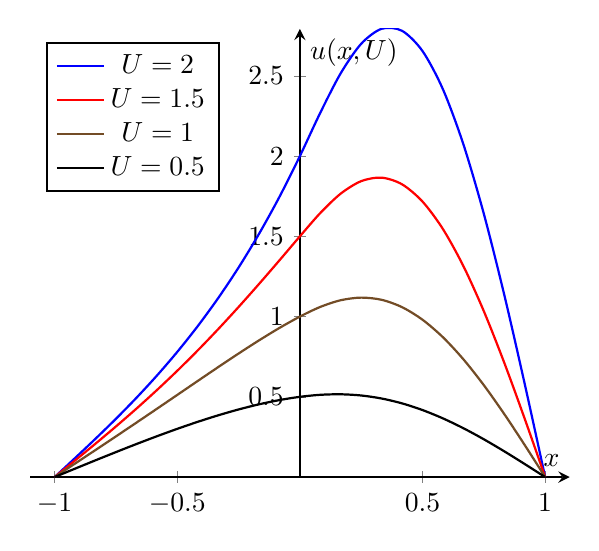
\begin{tikzpicture}
\def\alfa{2}
\begin{axis}[xlabel={$x$},ylabel={$u(x,U)$}
,domain=-1:1,axis x line=middle, axis y line=middle
,xmin=-1.1,xmax=1.1,legend pos=north west,thick,smooth]
\foreach \uu in {2,1.5,1,0.5} {
    \addplot+[no marks] {\uu*(1-6/5*abs(x)^2-1/10*abs(x)^3+3/8*abs(x)^4-3/40*abs(x)^5)+\alfa*(\uu^2)*x*(2/5-abs(x)^2+3/4*abs(x)^3-3/20*abs(x)^4)+\alfa^2*(\uu)^3*(2/15*abs(x)^2-4/15*abs(x)^3+1/6*abs(x)^4-1/30*abs(x)^5)};
\addlegendentryexpanded{$U=\uu$};
};
\end{axis}
\end{tikzpicture}
&
\parbox[b]{0.45\linewidth}{\caption{\label{fig:nonlinsm}%
nonlinear slow manifold for Burgers' \pde~\eqref{eq:burgers} for viscosity \(\nu=1\) and nonlinearity \(\alpha=2\)\,.  
Drawn is the slow manifold~\(u(x,U)\) for representative amplitudes \(U=\tfrac12,1,\tfrac32,2\) to show the larger deformation at larger amplitudes.  
This approximation to the slow manifold was computed to errors~\Ord{\gamma^3+\alpha^3} and evaluated at full coupling \(\gamma=1\)\,.
}}
\end{tabular}
\end{figure}

Centre manifold theory~\cite[Ch.~4, e.g.]{Carr81, Roberts2014a} was designed for nonlinear problems.
Thus it also applies here to the nonlinear Burgers' \pde~\eqref{eq:burgers} similarly modelled with two intervals on the domain \(-1<x<1\)\,.
For example, modified computer algebra~\cite[Ch.~14]{Roberts96a, Roberts2014a} \ajr{Code needs to be checked??} constructs the slow manifold plotted in Figure~\ref{fig:nonlinsm} on which the nonlinear evolution is
\begin{equation*}
\dot U=-(3\gamma+\tfrac35\gamma^2)U-\tfrac1{15}\gamma^2\alpha^2U^3
+\Ord{\gamma^3+\alpha^3}.
\end{equation*}
The nonlinear advection of Burgers' \pde\ generates steeper gradients (Figure~\ref{fig:nonlinsm}) that enhance the decay as expressed by the cubic nonlinearity in this evolution equation for amplitude~\(U(t)\).

Key properties of this example are also exhibited in the application of the approach to the more general spatial discretisations discussed by subsequent sections: an analogous inter-element coupling engenders an emergent slow manifold; the linearised operator is self-adjoint; the first iteration constructs a cubic spline; and the resultant model at full coupling has attractive properties.






\section{Motivation}\label{sec:motive}
The choice of a piecewise linear leading approximation, in contrast to the usual piecewise constant one \cite[]{Roberts98a, Roberts00a, Roberts2011a}, is motivated by two factors: firstly, the empirical observation
that linear approximation is frequently employed in practice as a cheap means of interpolating between grid-point values;
and secondly, as the consequence of an application of the Rayleigh--Ritz theorem.
Consider a general dynamical system of the form
\begin{eqnarray}
\dot{\uv} = {\cL}{\uv}+{\cN}({\uv})\,,
\label{eq:nonlin:gen}
\end{eqnarray}
where it is pre-supposed for convenience that ${\cN}({\vec 0})={\vec 0}$. 
The slow manifold approximation to the dynamics of the linearised system
\begin{eqnarray}
 \dot{{\uv}}={\cL}{\uv}
\label{eq:lin:gen}
\end{eqnarray}
about ${\uv}={\vec 0}$ is then parameterised as
\begin{eqnarray}
{\uv} = V{\sv}\,, && \dot{{\sv}} = \Lambda{\sv}\,,
\end{eqnarray}
whereupon $V\Lambda{\sv}={\cL}V{\sv}$ for arbitrary ${\sv}$.
Observe that the particular choice of $\Lambda=\mbox{diag}(\lambda_1,\lambda_2,\ldots)$ uncouples this relation into the components
${\cL}{\vv}_j=\lambda{\vv}_j$, where $V=\begin{bmatrix} {\vv}_1&{\vv}_2&\cdots \end{bmatrix}$.

Now, when ${\cL}$ is self-adjoint, the Rayleigh--Ritz theorem is that $\lambda_j = R({\vv}_j)$ for the Rayleigh quotient 
\[ R({\vv}) = \frac{\langle{\vv},{\cL}{\vv}\rangle}{\|{\vv}\|^2}\,.\]
 It can further be shown, upon perturbing ${\vv}_j$ to ${\uv}={\vv}_j+\epsilon{\vec w}$,
that $R({\uv})=\lambda_j+\Ord{\epsilon^2}$.
%This provides support for the general expansions
%\begin{eqnarray}
%{\uv} \sim V{\sv}+\epsilon{\vec w}_1+\epsilon^2{\vec w}_2+\ldots\,,
%&& 
%\dot{\uv} \sim V\Lambda{\sv}+\epsilon{\gv}_1+\epsilon^2{\gv}_2+\ldots\,,
%\end{eqnarray}
%for the nonlinear dynamical system~\eqref{eq:nonlin:gen}.
The slow manifold is based upon the slow subspace spanned by the slow eigenvectors, and the evolution on the slow manifold corresponds to eigenvalues of the linearisation.
Hence the Rayleigh--Ritz quotient suggests that the more accurate we make a linear subspace approximation to the field~\(u(x,t)\), the more accurate the evolution on the slow manifold.
Consequently, Section~\secref{lin} develops a piecewise linear and continuous subspace approximation to the field.






\section{Linearisation establishes the existence of a closure}\label{sec:lin}

We use centre manifold theory \cite[e.g.]{Carr81, Haragus2011} to establish the in-principle existence and emergence of an exact closure to the dynamics of  \pde{}s in the class~\eqref{eq:genpde}.
Centre manifold theory is based upon an equilibrium or subspace of equilibria, and follows primarily from the spectrum of the linearised dynamics \cite[e.g.]{Roberts2014a}.

To find useful equilibria we embed the \pde~\eqref{eq:genpde} in a wider class of problems.
First partition the spatial domain into the \(N\)~intervals between the grid points \(x=X_j\)\,: let the interval \(\XX_j=\{x\mid X_{j-1}<x<X_j\}\) and denote the punctured domain \(\tilde\XX:=\XX\backslash\{X_0,X_1,\ldots,X_N\}\).
For definiteness take the boundary conditions on the field~\(u(x,t)\) to be that it is \(L\)-periodic in space.
Then use \(u_j(x,t)\)~to denote solutions of the \pde~\eqref{eq:genpde} on the interval~\(\XX_j\), and reserve \(u(x,t)\), over~\XX\ or~\(\tilde\XX\) as appropriate, to denote the union over all intervals of such solutions.
To restore the original \pde~\eqref{eq:genpde} over the whole domain~\XX\ we couple the fields on each interval together.
By controlling the information flow between intervals, we embed the original \pde\ over the whole domain to a useful base problem.
The coupling conditions are  
\begin{subequations}\label{eqs:cc}%
\begin{eqnarray}
&&[u]_{X_j^-}^{X_j^+}=0
\quad\text{and }
\label{eq:ccc}
\\&&
[\nu u_x]_{X_j^-}^{X_j^+}=\frac{C(\gamma)}H\left[
(\nu u)|_{X_{j+1}^-} -(\nu u)|_{X_{j}^+}
+(\nu u)|_{X_{j-1}^+} -(\nu u)|_{X_{j}^-}\right],\qquad
\label{eq:ccj}
\end{eqnarray}
\end{subequations}
where coefficient \(\nu(x)=F'(u_x)\) is the effective diffusivity at each point in~\(\tilde\XX\), via the gradient~\(u_x\),
and where the factor~\(C(\gamma)\) is some smooth function such that \(C(0)=1\) and \(C(1)=0\) (typically \(C(\gamma):=1-\gamma\)).

\begin{lemma}[equilibria] \label{thm:equil}
The \pde~\eqref{eq:genpde} on domain~\(\tilde\XX\) with coupling conditions~\eqref{eqs:cc} possesses an \(N\)-dimensional subspace~\EE\ of equilibria, parametrised by \(\Uv=(U_1,U_2,\ldots,U_N)\), for parameters \(\alpha=\gamma=0\) of piecewise linear solutions~\(u^*(x)\) such that on the \(j\)th~interval the field 
\begin{equation}
u_j^*(x)=(1-\xi)U_{j-1}+\xi U_j
\quad\text{where }\xi=(x-X_{j-1})/H
\label{eq:equil}
\end{equation}
is a local scaled space variable.
\end{lemma}

\begin{proof} 
With nonlinearity \(\alpha=0\) the \pde~\eqref{eq:genpde} takes the form \(u_t=F(u_x)_x\)\,.
For the piecewise linear field~\eqref{eq:equil}, the gradient \(u^*_x=(U_j-U_{j-1})/H\) is constant on each~\(\XX_j\). 
Hence \(F(u^*_x)\) is constant on each~\(\XX_j\).
Consequently, \(F(u^*_x)_x=0\) on~\(\tilde\XX\), giving an equilibria of the \pde\ on~\(\tilde\XX\).

From the field~\eqref{eq:equil},  \(u^*_j(X_j^-)=U_j=u^*_{j+1}(X_j^+)\) and hence \(u^*(x)\)~is continuous at~\(X_j\) to satisfy the coupling condition~\eqref{eq:ccc}.

Lastly, consider the condition~\eqref{eq:ccj} on the jump in the derivative.
For the field~\eqref{eq:equil}, the gradient is \(u^*_x=(U_j-U_{j-1})/H\) so, in terms of the constants 
\begin{equation}
\nu_j:=F'(u^*_{jx})=F'\big(\tfrac{U_j-U_{j-1}}H\big),
\label{eq:nuj}
\end{equation} 
the jump in gradient 
\begin{eqnarray*}
[\nu u^*_x]_{X_j^-}^{X_j^+}
&=&\nu_{j+1}\frac{U_{j+1}-U_j}H-\nu_j\frac{U_j-U_{j-1}}H
\\&=&\frac1H(\nu_{j+1}U_{j+1}-\nu_{j+1}U_j+\nu_jU_{j-1}-\nu_jU_j)
\\&=&\frac1H\left(\nu|_{X_{j+1}^-}u^*|_{X_{j+1}^-}
-\nu|_{X_{j}^+}u^*|_{X_{j}^+}
+\nu|_{X_{j-1}^+}u^*|_{X_{j-1}^+}
-\nu|_{X_{j}^-}u^*|_{X_{j}^-}\right)
\end{eqnarray*}
which is the required right-hand side of~\eqref{eq:ccj} for coupling parameter \(\gamma=0\) (as \(C(0)=1\)).
Hence, the piecewise linear fields~\eqref{eq:equil}, with \(\alpha=\gamma=0\), are equilibria for all~\Uv, and clearly form an \(N\)-D~subspace.
\end{proof}

The spectrum comes from the linearised dynamics around each of the equilibria~\EE.
Seek solutions \(u=u^*(x)+\hat u(xt)\) of the general \pde~\eqref{eq:genpde} where \(\hat u(x,t)\)~denotes a small perturbation to the equilibrium~\eqref{eq:equil}. 
Use \(\hat u_j(x,t)\) as a synonym for~\(\hat u(x,t)\) on the \(j\)th~interval~\(\XX_j\).
Then for parameters \(\alpha=\gamma=0\) and small~\(\hat u\), the \pde~\eqref{eq:genpde} linearises to
\begin{subequations}\label{eqs:lin}%
\begin{equation}
\hat u_t=F'(u^*_x)\hat u_{xx}=\nu(x)\hat u_{xx}\quad\text{on }\tilde\XX; 
\quad\text{that is,}\quad 
\hat u_{jt}=\nu_j\hat u_{jxx}\quad\text{on }\XX_j.
\label{eq:pdelin}
\end{equation}
The coupling conditions~\eqref{eqs:cc} are linear so they are 
\([\hat u]_{X_j^-}^{X_j^+}=0\) and \([\nu\hat u_x]_{X_j^-}^{X_j^+}=\frac1H\big[
(\nu\hat  u)|_{X_{j+1}^-} -(\nu\hat  u)|_{X_{j}^+}
+(\nu\hat  u)|_{X_{j-1}^+} -(\nu\hat  u)|_{X_{j}^-}\big]\);
%\begin{eqnarray*}
%&&[\hat u]_{X_j^-}^{X_j^+}=0
%\quad\text{and }
%%\label{eq:ccc}
%\\&&
%[\nu\hat u_x]_{X_j^-}^{X_j^+}=\frac1H\left[
%(\nu\hat  u)|_{X_{j+1}^-} -(\nu\hat  u)|_{X_{j}^+}
%+(\nu\hat  u)|_{X_{j-1}^+} -(\nu\hat  u)|_{X_{j}^-}\right],
%%\label{eq:ccj}
%\end{eqnarray*}
that is,
\begin{eqnarray}
&&\hat u_{j+1}(X_j)=\hat u_j(X_j)
\quad\text{and }
\label{eq:ccclin}
\\&&
\nu_{j+1}\hat u_{j+1,x}(X_j)-\nu_j\hat u_{jx}(X_j)
\nonumber\\&&{}
=\frac1H\left[
\nu_{j+1}\hat u_{j+1}(X_{j+1}) -\nu_{j+1}\hat u_{j+1}(X_{j})
+\nu_j\hat  u_j(X_{j-1}) -\nu_j\hat  u_j(X_{j})\right].
\qquad\label{eq:ccjlin}
\end{eqnarray}
\end{subequations}
The next lemma certifies that this linearised system is self-adjoint and so we need only seek real eigenvalues in the spectrum.

\begin{lemma}[self-adjoint] \label{thm:sa}
The differential operator appearing in~\eqref{eqs:lin}, namely \(\cL=\nu\DD x{}\) on~\(\tilde\XX\) subject to~\eqref{eq:ccclin}--\eqref{eq:ccjlin} and for \(L\)-periodic solutions, is self-adjoint upon using the usual inner product \(\left<v,u\right>:=\int_{\tilde\XX} vu\,dx\)\,.
\end{lemma}

\begin{proof} 
Straightforwardly use integration by parts (remembering that \(\nu\)~is piecewise constant):
\begin{eqnarray*}
\left<v,\cL u\right>
&=&\int_{\tilde\XX}v\nu u_{xx}\,dx
\\&=&\sum_j \left[\nu v u_x-\nu u v_x\right]_{X_{j-1}^+}^{X_j^-}
+\int_{\tilde\XX}\nu v_{xx}u\,dx
\\&=&\sum_j \left[ 
\nu_j v_j(X_j^-) u_{jx}(X_j^-)
-\nu_j u_j(X_j^-) v_{jx}(X_j^-) 
\right.\\&&\quad\left.{}
-\nu_j v_j(X_{j-1}^+) u_{jx}(X_{j-1}^+)
+\nu_j u_j(X_{j-1}^+) v_{jx}(X_{j-1}^+) \right]
+\left<\cL v, u\right>
\\&&(\text{using the continuity~\eqref{eq:ccclin} and }U_j:=u(X_j^\pm),\ V_j:=v(X_j^\pm)\,)
\\&=&\sum_j \left[ 
\nu_j V_j u_{jx}(X_j^-)
-\nu_j U_j v_{jx}(X_j^-) 
\right.\\&&\quad\left.{}
-\nu_j V_{j-1} u_{jx}(X_{j-1}^+)
+\nu_j U_{j-1} v_{jx}(X_{j-1}^+) \right]
+\left<\cL v, u\right>
\\&&(\text{reindexing the last two terms in the sum, }j\mapsto j+1)
\\&=&\sum_j \left[ 
V_j \nu_j u_{jx}(X_j^-)
-U_j \nu_j v_{jx}(X_j^-) 
\right.\\&&\quad\left.{}
- V_{j} \nu_{j+1} u_{j+1,x}(X_{j}^+)
+ U_{j} \nu_{j+1} v_{j+1,x}(X_{j}^+) \right]
+\left<\cL v, u\right>
\\&&(\text{replacing two pairs of terms via coupling~\eqref{eq:ccjlin}})
\\&=&\sum_j \left\{ 
-V_j \tfrac1H\left[ \nu_{j+1}U_{j+1} -\nu_{j+1}U_{j}
+\nu_jU_{j-1} -\nu_jU_j \right]
\right.\\&&\quad\left.{}
+ U_{j}\tfrac1H \left[ \nu_{j+1}V_{j+1} -\nu_{j+1}V_{j}
+\nu_jV_{j-1} -\nu_jV_j \right] \right\}
+\left<\cL v, u\right>
\\&&(\text{cancelling all terms in }U_jV_j)
\\&=&\sum_j \tfrac1H\left\{ 
-V_j\nu_{j+1}U_{j+1} 
-V_j\nu_jU_{j-1} 
+ U_{j} \nu_{j+1}V_{j+1} 
+U_j\nu_jV_{j-1}   \right\}
\\&&\quad{}
+\left<\cL v, u\right>
\\&&(\text{reindexing 2nd and 4th terms in the sum, }j\mapsto j+1)
\\&=&\sum_j 0
+\left<\cL v, u\right> =\left<\cL v, u\right>.
\end{eqnarray*}
Hence, as required, the linear operator in the linearised system~\eqref{eqs:lin} is self-adjoint.
\end{proof}

We turn to determining the spectrum of the general linearised system~\eqref{eqs:lin}: first, the zero eigenvalues; and second, the non-zero eigenvalues.
Because of the \(N\)-D~subspace of equilibria~\EE\ the linearised system must have \(N\)~eigenvalues of zero.
Corresponding basis eigenfunctions may be chosen to be 
\begin{equation*}
\phi_j(x)=\max(0,1-|x-X_j|/H)
\end{equation*}
so the equilibria~\eqref{eq:equil} may be written \(u^*=\sum_j \phi_j(x)U_j\)\,.
The localised triangular shape of these basis functions, incidentally,  many will recognise as the fundamental ``shape function'' often invoked in the finite element method \cite[e.g.]{OLeary08, ??}.
For the linearised \pde~\eqref{eq:pdelin} any eigenfunction corresponding to an eigenvalue of zero must be linear on each~\(\XX_j\), and the continuity~\eqref{eq:ccclin} then guarantees there are no other eigenfunctions than those identified.
By self-adjointness, there are no generalised eigenfunctions.
Thus the slow subspace of the system~\eqref{eqs:lin} is \(N\)-D, namely~\EE.

For rigorous theory we notionally adjoin the two trivial dynamical equations \(\alpha_t=\gamma_t=0\) to the linearised system~\eqref{eqs:lin}.
Then,  as \(\alpha=\gamma=0\)\,, the equilibria~\eqref{eq:equil} are~\((0,0,u^*(x))\).
Thus strictly there are two extra zero eigenvalues associated with the trivial \(\alpha_t=\gamma_t=0\)\,, and the corresponding slow subspace of each equilibria is \((N+2)\)-D.
Except for issues associated with the domain of validity, for simplicity we do not explicitly include these two trivial dynamical equations nor their eigenvalues in the following, but consider them implicit.

\begin{lemma}[exponential dichotomy] \label{thm:dicho}
Provided function~\(F\) in the \pde~\eqref{eq:genpde} is monotonic increasing with \(F'\geq\nu_{\min}>0\)\,, then  the operator\(\cL=\nu\DD x{}\) on~\(\tilde\XX\) subject to~\eqref{eq:ccclin}--\eqref{eq:ccjlin} and for \(L\)-periodic solutions has \(N\)~zero eigenvalues and all other eigenvalues are negative and bounded away from zero by \(\lambda\leq-\nu_{\min}\pi^2/H^2\).
\end{lemma}

\begin{proof} 
The precisely \(N\)~zero eigenvalues are established in the two paragraphs before the statement of the lemma.

The Self-adjoint Lemma~\ref{thm:sa} establishes all eigenvalues of~\(\cL\) are real. 
Let \(\lambda\)~be a non-zero eigenvalue and \(v(x)\)~be a corresponding eigenfunction.
Then \(v\perp\EE\) by self-adjointness of~\cL, and, as usual,
\begin{equation*}
(-\lambda)\|v\|^2
=-\lambda\left<v,v\right>
=\left<v,-\lambda v\right>
=\left<v,-\cL v\right>.
\end{equation*}
Decompose the eigenfunction into \(v(x)=\tilde v(x)+\check v(x)\) where \(\check v(x)\)~is piecewise linear, continuous, and satisfies \(\check v(X_j)=v(X_j)\), so that \(\tilde v\)~is also continuous and \(\tilde v(X_j)=0\)\,.
Since \(\check v\in\EE\), so \(\cL\check v=0\) (the check accent is to remind us of the piecewise linear nature of~\(\check v\)).
Consequently, 
\(-\lambda\|v\|^2
=\left<v,-\cL v\right>
=\left<\tilde v+\check v,-\cL\tilde v-\cL\check v\right>
=\left<\tilde v,-\cL\tilde v\right>
+\left<\check v,-\cL\tilde v\right>
+\left<\tilde v,-\cL\check v\right>
+\left<\check v,-\cL\check v\right>\);
but \(\cL\check v=0\) so the last two terms in this sum are zero; and
by self-adjointness \(\left<\check v,-\cL\tilde v\right>=\left<\cL\check v,-\tilde v\right>=\left<0,-\tilde v\right>=0\) so the second term is also zero.
Thus we proceed to derive the inequality
\begin{eqnarray*}
-\lambda\|v\|^2&=&\left<\tilde v,-\cL\tilde v\right>
=\int_{\tilde\XX}-\nu\tilde v\tilde v_{xx}\,dx
\\&=&\sum_j\left[-\nu\tilde v\tilde v_x\right]_{X_{j-1}^+}^{X_j^-}
+\int_{\tilde\XX}\nu\tilde v_x^2\,dx
\quad(\text{integrating by parts})
\\&=&\sum_j 0
+\int_{\tilde\XX}\nu\tilde v_x^2\,dx
\quad(\text{using }\tilde v(X_j^-)=\tilde v(X_j^+)=0)
\ajr{I have an uncomfortable feeling about this as we have not used the jump in derivative condition---unless we have implicitly in check v component??}
\\&\geq&\nu_{\min}\int_{\tilde\XX}\tilde v_x^2\,dx
\quad(\text{as }\nu(x)\geq \nu_{\min}>0).
\end{eqnarray*}

Now relate this inequality to the spatially homogeneous problem.
Let \(\cL_1=\DD x{}\)~denote the linear operator with coupling conditions appearing in~\eqref{eqs:lin} for the special case of \(\nu(x)=\nu_j=1\) for all~\(x\) and~\(j\).
Then by the reverse of the argument of the previous paragraph,
\begin{equation*}
\int_{\tilde\XX}\tilde v_x^2\,dx
=\cdots=\left<\tilde v,-\cL_1\tilde v\right>
=\cdots=\left< v,-\cL_1 v\right>
\geq -\lambda_1\|v\|^2.
\end{equation*}
where \(\lambda_1\)~denotes the smallest magnitude, non-zero, eigenvalue of~\(\cL_1\).
The inequality is justified by the Rayleigh--Ritz theorem which asserts \(-\lambda_1=\min_{w\perp\EE} \left<w,-\cL_1w\right>/\|w\|^2\).
By the next Lemma~\ref{lem:hs}, \(-\lambda_1\geq\pi^2/H^2\), and hence all eigenvalues satisfy \(-\lambda\geq\nu_{\min}(-\lambda_1)\geq\nu_{\min}\pi^2/H^2\) as required.
\end{proof}



\begin{lemma}[spatially homogeneous spectrum] \label{lem:hs}
The non-zero eigenvalues of the differential operator \(\DD x{}\) on~\(\tilde\XX\) with coupling conditions~\eqref{eq:ccclin}--\eqref{eq:ccjlin} when \(\nu_j=1\) all satisfy \(\lambda\leq-\pi^2/H^2\).
\end{lemma}

\begin{proof} 
For the spatially homogeneous problem~\eqref{eqs:lin}, set \(\nu(x)=\nu_j=1\)\,. 
Seeking solutions \(e^{\lambda t}v(x)\) leads to the \ode\ \(\lambda v=v''\) on~\(\tilde\XX\).
As a constant coefficient \ode, and for eigenvalues \(\lambda=-\kappa^2/H^2\) for some nondimensional wavenumber~\(\kappa\geq0\) to be determined, its general solutions are of the form \(v_j=A_j\cos[\kappa(x-X_{j-1})/H]+B_j\sin[\kappa(x-X_{j-1})/H]\) for coefficients~\(A_j\) and~\(B_j\) determined by the coupling conditions~\eqref{eq:ccclin}--\eqref{eq:ccjlin}. 
Consequently, the derivative \(v_{jx}=-\frac{A_j\kappa}H\sin[\kappa(x-X_{j-1})/H]+\frac{B_j\kappa}H\cos[\kappa(x-X_{j-1})/H]\).

Let's consider the spatial map \((A_j,B_j)\mapsto(A_{j+1},B_{j+1})\).
Continuity~\eqref{eq:ccclin} at \(x=X_j\) requires 
\begin{equation*}
A_{j+1}=A_j\cos\kappa+B_j\sin\kappa=cA_j+sB_j
\end{equation*}
where for brevity in this proof, let \(c:=\cos\kappa\) and \(s:=\sin\kappa \)\,.
The derivative jump~\eqref{eq:ccjlin} at \(x=X_j\) requires
\begin{equation*}
\frac\kappa H B_{j+1}+A_j\frac\kappa H s-B_j\frac\kappa H c
=\frac{C(\gamma)}H\left[cA_{j+1}+sB_{j+1} -2A_{j+1} +A_j \right],
\end{equation*}
where we include the factor~\(C(\gamma)\) for a little more generality;
that is,
\begin{equation*}
(c-2)CA_{j+1}+(Cs-\kappa)B_{j+1}+(C-s\kappa)A_j+c\kappa B_j=0\,.
\end{equation*}
Dividing by~\(C\), and in terms of \(\kappa'=\kappa/C\)\,, gives the equivalent
\begin{equation*}
(c-2)A_{j+1}+(s-\kappa')B_{j+1}+(1-s\kappa')A_j+c\kappa'B_j=0\,.
\end{equation*}
Considering together the two equations, this spatial map has solutions \((A_j,B_j)\propto \mu^j\) for some multiplier~\(\mu\) only if the determinant
\begin{eqnarray}&&
\det\begin{bmatrix} \mu-c&-s\\
\mu (c-2)+1-s\kappa'&\mu(s-\kappa')+c\kappa' \end{bmatrix}=0\,;
\nonumber
\\&&\text{that is,}\quad
\mu^2-2\frac{c\kappa'-s}{\kappa'-s}\mu+1=0\,.
\end{eqnarray}
%Hence the two possible multipliers must have product one, which reflects the left-right spatial symmetry in the linear problem~\eqref{eqs:lin}.
Hence the two possible multipliers of the spatial map are 
\begin{equation*}
\mu=\beta\pm\sqrt{\beta^2-1}\quad\text{for }\beta=\frac{s-c\kappa'}{s-\kappa'}\,.
\end{equation*}
Consequently, \(|\beta|>1\) is not possible as then there are two (real) multipliers: one of which has magnitude greater than one representing structures growing exponentially quickly to the right; and one of which has magnitude less than one representing structures growing exponentially quickly to the left.
The only allowable cases occur for \(|\beta|\leq1\) when the multipliers are complex of magnitude \(|\mu|=1\) and so characterise periodic structures in space.
Since \(\kappa'-s=\kappa/C(\gamma)-\sin\kappa\geq0\)\,, the requirement \(|\beta|\leq1\) becomes \(s-\kappa'\leq c\kappa'-s\leq\kappa'-s\)\,; that is, \(2s-\kappa'\leq c\kappa'\leq\kappa'\).
But the right-hand inequality is always satisfied as \(c=\cos\kappa\)\,, but the left-hand inequality requires \(2s\leq(1+c)\kappa'\), that is, \(s/(1+c)\leq\kappa'/2\)\,.
Recalling \(s=\sin\kappa\) and \(c=\cos\kappa\) this requirement becomes
\begin{equation}
\tan\frac\kappa2\leq\frac\kappa{2C}\,.
\label{eq:kappa}
\end{equation}
\begin{figure}
\centering
\begin{tabular}{cc}
\tikzsetnextfilename{spectrum}
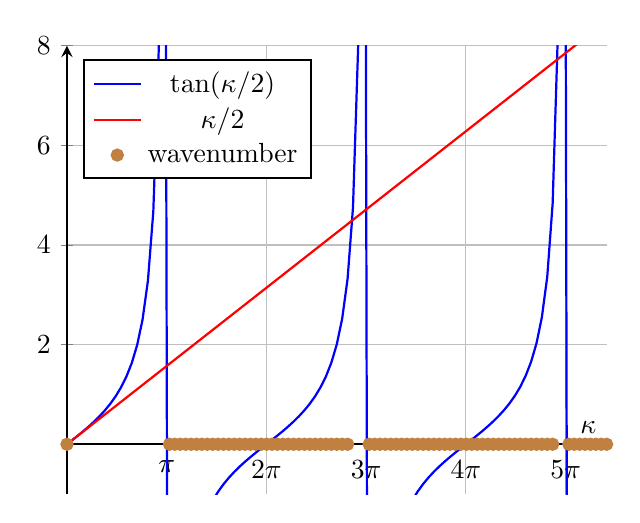
\begin{tikzpicture}
\begin{axis}[ xlabel={$\kappa$}
  ,axis x line=middle,axis y line=middle
  ,thick,grid,samples=101
  ,ymin=-1,ymax=8 ,domain=0:17
  ,xtick={3.1416,6.2832,9.4248,12.5664,15.7080}
  ,xticklabels={$\pi$,$2\pi$,$3\pi$,$4\pi$,$5\pi$}
%  ,legend pos=outer north east
  ,legend pos=north west
  ] 
\addplot [blue,no marks] {tan(deg(x)/2)}; 
\addlegendentry{$\tan(\kappa/2)$};
\addplot [red,no marks,samples=2] {x/2}; 
\addlegendentry{$\kappa/2$};
\addplot [brown,only marks,mark=*] {0-99*(x/2<tan(deg(x)/2))};
\addlegendentry{wavenumber};
\end{axis}
\end{tikzpicture}
&
\parbox[b]{0.4\linewidth}{\caption{\label{fig:leaspec}%
The linearised ($\gamma=0$, \(C=1\)) spectrum determined by the spectral requirement~\eqref{eq:kappa}.
The thick lines along the $\kappa$-axis indicate regions of spatial wavenumbers for which the corresponding spatial structures are bounded for all space.}}
\end{tabular}
\end{figure}%
As illustrated by Figure~\ref{fig:leaspec}, for the specific case of the linearised problem~\eqref{eqs:lin} for which \(C(0)=1\)\,, the smallest allowable nonzero nondimensional wavenumber is \(\kappa=\pi\)\,.
Hence the smallest magnitude nonzero eigenvalue is\({}\leq-\pi^2/H^2\) as required.
\end{proof}

Comment on filling the gap as \(C\)~decreases??


\begin{theorem}[slow manifold]
In a neighbourhood of the subspace~\EE\ there exists an \(N\)-D slow manifold that is emergent with transients roughly\({}\propto\exp(-\nu_{\min}\pi^2/H^2\,t)\).
\end{theorem}

\begin{proof} 
??
\end{proof}






\subsection*{Reconsider the following??}
Burgers' equation~\eqref{eq:burgers} linearises to equation~\eqref{eq:lin:gen} for $\alpha=0$, with the linear operator
${\cL}=\nu\DD x{}$. It can be shown that ${\cL}$ is self-adjoint under any of these external boundary conditions:
\(L\)-periodic; Dirichlet ($u(0,t)=u(L,t)=0$); or Neuman ($u_x(0,t)=u_x(L,t)=0$). We have chosen the first
condition for convenience.
The linear system has two eigenmodes corresponding to eigenvalue $\lambda=0$, namely
\begin{eqnarray}
  v = 1\,, && v = x\,, 
\end{eqnarray}
and general eigenmodes for $\lambda=-\nu k^2<0$ of the form
\begin{eqnarray}
 v = e^{-\nu k^2 t\pm ikx}\,.&&
\end{eqnarray}
Hence, any peicewise--linear approximation to $u$ is an equilibrium solution of the linearised system.
We choose a continuous approximation that is aligned at the internal grid-points $X_j=jH$, $j=1,2,\ldots,N-1$, namely
\begin{eqnarray}
     \hat{u}_{0} = \sum_{j=1}^{N}\chi_j(x)(\xi U_j+(1-\xi)U_{j-1})
% = \sum_{j=1}^{N}\chi_j(\xi+(1-\xi)\sigma^{-1})U_j
\,,
\label{eq:uhat0}
\end{eqnarray}
with indicator $\chi_j(x)=1$ (else 0) for $X_{j-1}\le x<X_j$, and dimensionless coordinate
$\xi(x)=\sum_{j=1}^{N}\chi_j(x)(x-X_{j-1})/H$. This enforced continuity is represented by internal coupling conditions
(\cc{}s) of the form 
\begin{eqnarray}
   [\hat{u}]_j = 0 && \mbox{for } j=1,2,\ldots,N-1\,,
\label{eq:cont-cond}
\end{eqnarray}
where $ [u]_j := \lim_{\epsilon\rightarrow 0^{+}} u(X_j+\epsilon,t)-u(X_j-\epsilon,t)$
represents the spatial jump in $u$ across the boundary between the $j$th and $(j+1)$th intervals.

Unfortunately, this continuity does not hold for the first spatial derivative, since it can be shown that
$[\D x{\hat{u}_{0}}]_j=\delta^2U_j/H$. Hence, we introduce a homotopic smoothing parameter $\gamma$
($0\le\gamma\le 1$),
and enforce the additional \cc{}s: %smoothness condition that
\begin{eqnarray}
   [\hat{u}_x]_j = \frac{1-\gamma}{H}\left.\delta^2\hat{u}\right|_{X_j} && \mbox{for } j=1,2,\ldots,N-1\,,
\label{eq:smooth-cond}
\end{eqnarray}
such that smooth approximations are found in the limit as $\gamma\rightarrow 1$.
Consequently, the state-space is now extended to $(u,\alpha,\gamma)$, for which $(\hat{u}_{0},0,0)$ is
an equilibrium of equation~\eqref{eq:burgers}.  

We now demonstrate that the system will be robust to nonlinear perturbations about this equilibrium.
We seek the spatial stability over $\XX$ of the eigenmode
\begin{eqnarray}
v = \sum_{j=1}^{N}\chi_j \Re\left(a_j e^{i\kappa\xi}\right)\,,
\end{eqnarray}
for some fixed, nondimensionalised wavenumber $\kappa=kH$, and 
arbitrary, time--varying coefficients $a_j=A_j+iB_j$. 
The continuity condition~(\ref{eq:cont-cond}) now implies that
\begin{eqnarray}
\Re\left(a_{j+1} - a_j e^{i\kappa}\right) = 0\,.
\end{eqnarray}
Similarly, the smoothness condition~(\ref{eq:smooth-cond}) implies that 
\begin{eqnarray}
-\kappa \Im\left(a_{j+1} - a_j e^{i\kappa}\right) =  
(1-\gamma)\Re\left(a_{j+1} e^{i\kappa} + a_j - 2 a_j e^{i\kappa}\right)\,.
\end{eqnarray}
In coefficient form, the update from the $j$th to $(j+1)$th interval is
\begin{eqnarray}
\left[\begin{array}{cc}
1 & 0\\
fc & 1-fs\\
\end{array}\right]
\left[\begin{array}{c}
A_{j+1}\\
B_{j+1}\\
\end{array}\right]
=
\left[\begin{array}{cc}
c & -s\\
s+f(2c-1) & c-2fs\\
\end{array}\right]
\left[\begin{array}{c}
A_{j}\\
B_{j}\\
\end{array}\right]\,,
\end{eqnarray}
where $c+is=e^{i\kappa}$ and $f=(1-\gamma)/\kappa$.
Putting $a_{j+1}=\mu a_j$ then leads to the characteristic equation
\begin{eqnarray}
\mu^2-2\frac{c-fs}{1-fs}\mu+1 = 0\,,
\end{eqnarray}
with characteristic roots given by
\begin{eqnarray}
\mu & = & \beta\pm\sqrt{\beta^2-1}
\hspace*{5mm}\mbox{for } 
\beta~=~\frac{c-fs}{1-fs}\le 1\,.
\end{eqnarray}
Consequently, there are three distinct stability regimes governed by $\beta$:
\begin{enumerate}
\item $|\beta|<1$, which gives rise to complex roots with $|\mu|=1$ ({\em marginally stable}). 
This includes the limiting case of $\gamma=1$ ($f=0$), for which
$\mu=c\pm is=e^{\pm i\kappa}$.

\item $\beta=\pm 1$, corresponding to $\kappa=n\pi$, $n=0,1,2,\ldots$, 
which gives rise to a repeated, real root of $\mu=\pm 1$ ({\em marginally stable}).

\item $\beta<-1$, which gives rise to the two real roots $\mu<-1$ and $-1<\mu<0$
({\em saddle unstable}).
\end{enumerate}
The $\beta<-1$ regime comprises small regions of instability near $\kappa=(2n+1)\pi$,
$n=0,1,2,\ldots$, for which the eigenmode cannot persist unattenuated throughout space.
It can be shown that these forbidden regions obey
\begin{eqnarray}
\frac{\kappa}{2} <(1-\gamma)\tan\frac{\kappa}{2}\,, && \kappa\ne n\pi\,.
\label{eq:leaforbid}
\end{eqnarray}
Thus, at equilibrium ($\gamma=0$) there is an initial forbidden gap $\kappa\in(0,\pi)$ adjacent to the centre manifold
wavenumber $\kappa=0$ (see Figure~\ref{fig:leaspec}), indicating that transient solutions decay
 to the centre manifold at a rate of at least
$\lambda=-\nu k^2=-\frac{\nu\pi^2}{H^2}$. It is this gap that provides robustness to nonlinear perturbations
about the equilibrium within some suitable region in state-space.


\section{Nonlinear analysis}\label{sec:nonlin}

With the aid of  holistic equations~\eqref{eq:temporal} and \eqref{eq:spatial}, 
viz $u=\hat{u}$ and $\dot{\Uv}=\gv$, we rewrite
Burgers' equation~\eqref{eq:burgers} in the form
\begin{eqnarray}
 {\cM}(\hat{u},\gv) = {\cL}\hat{u}-\D {\Uv}{\hat{u}}\cdot\gv-\alpha\hat{u}\hat{u}_{x} = 0\,,
\label{eq:man}
\end{eqnarray}
where ${\cL}=\nu\DD {x}{}$ from Section~\secref{lin}. The linear analysis of that section is now extended
by considering perturbations about the equilibrium $(\hat{u},\gamma,\alpha)=(\hat{u}_{0},0,0)$.
%, where$\hat{u}_{0}=\sum_{j=1}^{N}\chi_j{\cI}_0 U_j$ with ${\cI}_0=\xi+(1-\xi)\sigma^{-1}$.
In particular, consider the power series
\begin{eqnarray}
  \hat{u} \sim \sum_{p=0}^{\infty}\sum_{q=0}^{\infty}\gamma^{p}\alpha^{q}\hat{u}^{(p,q)}\,,
&&
  \gv \sim \sum_{p=0}^{\infty}\sum_{q=0}^{\infty}\gamma^{p}\alpha^{q}\gv^{(p,q)}\,,
\label{eq:power}
\end{eqnarray}
where $\hat{u}^{(0,0)}=\hat{u}_{0}$ 
and $\gv^{(0,0)}=0$.
Substituting these expansions into
equation~\eqref{eq:man},  the terms $\hat{u}^{(p,q)}$ and $\gv^{(p,q)}$ are computed
subject to the \cc{}s \eqref{eq:cont-cond} and \eqref{eq:smooth-cond}.

To simplify this process algebraically, we follow the approach of \cite{Jarrad2001}:
without loss of generality, consider finite truncations of the power series subject to $p+q\le n$,
namely\footnote{In practice, other truncation schemes may be used;
for example, rectangular truncation: $p\le n$, $q\le m$.}
\begin{eqnarray}
   \hat{u}^{<n>} = \sum_{p=0}^{n}\sum_{q=0}^{n-p}\gamma^{p}\alpha^{q}\hat{u}^{(p,q)}\,,
&&
   \hat{u}_n = \sum_{p=0}^{n}\gamma^{p}\alpha^{n-p}\hat{u}^{(p,n-p)}\,.
\end{eqnarray}
Letting $\varepsilon^2=\gamma^2+\alpha^2$ for convenience\footnote{
This is merely an algebraic device; in practice, $\gamma$ and $\alpha$ need not be commensurate.}, we obtain
 $\hat{u}=\hat{u}^{<n>}+\Ord{\varepsilon^{n+1}}$ and
$\hat{u}^{<n>}=\hat{u}^{<n-1>}+\hat{u}_{n}$; 
likewise for $\gv^{<n>}$ and $\gv_n$.
It can then be shown that
\begin{eqnarray}
 {\cM}(\hat{u}^{<n>},\gv^{<n>}) = 
  {\cL}\hat{u}_n-\D {\Uv}{\hat{u}_0}\cdot\gv_n+{\cM}(\hat{u}^{<n-1>},\gv^{<n-1>})
+\Ord{\varepsilon^{n+1}}\,,
\end{eqnarray}
and hence the process is to iteratively solve
\begin{eqnarray}
 {\cM}(\hat{u}^{<n>},\gv^{<n>}) = 0+\Ord{\varepsilon^{n+1}}\,,
\end{eqnarray}
or, equivalently,
\begin{eqnarray}
{\cL}\hat{u}_n = \D {\Uv}{\hat{u}_0}\cdot\gv_n-{\cM}(\hat{u}^{<n-1>},\gv^{<n-1>})
%+\Ord{\varepsilon^{n+1}}
\,.
\label{eq:order-n}
\end{eqnarray}

Given $\hat{u}_0=\sum_{j=1}^{N}\chi_j(\xi+(1-\xi)\sigma^{-1})U_j$ 
where $\xi=\sum_{j=1}^{N}\chi_j(x-X_{j-1})/H$, the first-order pertubation terms 
can now be computed for $n=1$. 
Defining the backward difference $\nabla=1-\sigma^{-1}$, observe that
\begin{eqnarray}
\nu\hat{u}_{1}'' = \sum_{j=1}^{N}\chi_j\left[(\xi+(1-\xi)\sigma^{-1})g_{1,j}
   +\alpha(\xi+(1-\xi)\sigma^{-1})U_j.\frac{1}{H}\nabla U_j\right]\,.
\end{eqnarray}
Hence, spatially integrating twice gives
%\begin{eqnarray}
%\nu\hat{u}_{1}' & = & \sum_{j=1}^{N}\chi_j\left[c_j+ \frac{H}{2}(\xi^2-(1-\xi)^2\sigma^{-1})g_{1,j}
%\right.
%\nonumber\\
%&&  \left.{}+\frac{\alpha}{2}(\xi^2-(1-\xi)^2\sigma^{-1})U_j\,\nabla U_j\right]
%\end{eqnarray}
\begin{eqnarray}
\nu\hat{u}_{1} & = &  \sum_{j=1}^{N}\chi_j\left[d_j+H\xi c_j+\frac{H^2}{6}(\xi^3+(1-\xi)^3\sigma^{-1})g_{1,j}
\right.\nonumber\\
&& \left.{}+\frac{\alpha H}{6}(\xi^3+(1-\xi)^3\sigma^{-1})U_j\,\nabla U_j\right]\,.
\end{eqnarray}
Now, the continuity condition~\eqref{eq:cont-cond} ensures that $\hat{u}_n(X_j,t)=0$ for $n>0$,
since $\hat{u}_{0}(X_j,t)=U_j(t)=u(X_j,t)$. Hence, we solve for $d_j$ at $\xi=0$ and
$c_j$ at $\xi=1$, giving
\begin{eqnarray}
\nu\hat{u}_{1} & = &  \sum_{j=1}^{N}\chi_j\left[\frac{H^2}{6}(\xi^3+(1-\xi)^3\sigma^{-1}
-\xi\nabla-\sigma^{-1})g_{1,j}
\right.\nonumber\\
&& \left.{}+\frac{\alpha H}{6}(\xi^3+(1-\xi)^3\sigma^{-1}-\xi\nabla-\sigma^{-1})U_j\,\nabla U_j\right]\,.
\end{eqnarray}
It is convenient here to introduce interpolation operators, ${\cI}_0=\xi+(1-\xi)\sigma^{-1}$ and
${\cI}_1=\xi^3+(1-\xi)^3\sigma^{-1}-\xi\nabla-\sigma^{-1}$ (observe that ${\cI}_1''=6{\cI}_0/H^2$),
whence
\begin{eqnarray}
 \hat{u} = \sum_{j=1}^{N}\chi_j\left[{\cI}_0 U_j+\frac{H^2}{6\nu}{\cI}_1\dot{U}_j
+\frac{\alpha H}{6\nu}{\cI}_1 U_j\,\nabla U_j\right]+\Ord{\gamma^2+\alpha^2}\,,
\end{eqnarray}
since $\dot{U}_j=g_{1,j}+\Ord{\gamma^2+\alpha^2}$. 

Next, the value for $g_{1,j}$ can likewise be found
from the smoothness condition~\eqref{eq:smooth-cond}, namely
\begin{eqnarray}
\nu[\hat{u}_{1}']_{j} = -H\left(1+\frac{1}{6}\delta^2\right)g_{1,j} 
-\frac{\alpha}{3}\left(U_j.\mu\delta U_j+\mu\delta U_j^2\right)
= -\frac{\nu\gamma}{H}\delta^2 U_j\,,
\label{eq:g1}
\end{eqnarray}
giving
\begin{eqnarray}
  \dot{U}_j  = S\left[\frac{\nu\gamma}{H^2}\delta^2 U_j
-\frac{\alpha}{3H}U_j.\mu\delta U_j-\frac{\alpha}{3H}\mu\delta U_j^2
\right]+\Ord{\gamma^2+\alpha^2}\,,
\end{eqnarray}
where $S=(1+\delta^2/6)^{-1}$ is a non-local smoothing operator.
Observe that, apart $S$, this is just the mixture model~\eqref{eq:mixture}
with $\theta=\frac{2}{3}$. It turns out that this parameter value is exactly the critical value predicted by \cite{Fornberg73}
to be a necessary condition for the stability of numerical integration of the mixture model with $\nu=0$ and $\alpha=1$.
We demonstrate in Section~\secref{numeric} how this stability arises in low-dimensional models.

Higher order terms in $\hat{u}_n$  may be systematically computed by iteratively solving equation~\eqref{eq:order-n} after
having first computed $\gv_n$. The latter can be found by applying the weak solvability condition 
(see \cite{Jarrad2001}),
namely that the right-hand side of equation~\eqref{eq:order-n} must be orthogonal to the null-space of the adjoint
operator ${\cL}^{\dagger}$. Since ${\cL}$ is self-adjoint in this example, we can isolate the boundary between the
$j$th and $(j+1)$th intervals using the linear approximation
\begin{eqnarray}
  \hat{v}_0 = \chi_j\xi + \chi_{j+1}(1-\xi)\,,
\end{eqnarray}
which satisfies both the continuity condition~\eqref{eq:cont-cond} and the smoothness condition~\eqref{eq:smooth-cond}
(for $\gamma=0$). Thus, taking the inner product of equation~\eqref{eq:order-n} with $\hat{v}_0$ gives
rise to the solvability condition
\begin{eqnarray}
\left.\frac{\nu\gamma}{H}\delta^2\hat{u}_{n-1}\right|_{X_j} = HS^{-1}g_{n,j}
-\langle {\cM}(\hat{u}^{<n-1>},\gv^{<n-1>}), \hat{v}_0 \rangle\,.
\end{eqnarray}
Note that for $n=1$, this  reduces to equation~\eqref{eq:g1}, and
for $n>1$, the left-hand side is zero.

The higher order advection terms in $\alpha$ and the interactions between $\alpha$ and $\gamma$
rapidly become more complex. For example, the $\gamma\alpha$ terms are given by
\begin{eqnarray}
	g^{(1,1)}_{j} & = & \frac{1}{H}\left\{
  - \frac{1}{10}S\left(U_{j} S\mu\delta U_{j}\right)
  - \frac{1}{6}S\left(U_{j} \mu\delta U_{j}\right)
  + \frac{1}{10}S\left(SU_{j} \mu\delta U_{j}\right)
  \right.
\nonumber\\  
&& \left.- \frac{1}{5}S^{2}\left(U_{j} S\mu\delta U_{j}\right)
  + \frac{13}{30}S^{2}\left(U_{j} \mu\delta U_{j}\right)
  - \frac{1}{15}S^{3}\left(U_{j} \mu\delta U_{j}\right)
  \right.
\nonumber\\
&& \left.
  - \frac{1}{15}S^{3}\mu\delta U_{j}^2
  + \frac{7}{30}S^{2}\mu\delta U_{j}^2
  + \frac{2}{5}U_{j} S\mu\delta U_{j}
  - \frac{11}{30}S\mu\delta U_{j}^2
\right\}
\,.
\end{eqnarray}
In contrast, the terms purely in the homotopic parameter $\gamma$ represent smoothing corrections to the
diffusion; for example,
the coarse dynamics of the diffusion equation ($\alpha=0$)  obey 
\begin{eqnarray}
	\dot{U}_j & = & \frac{\nu\gamma}{H^2}S\delta^2 U _j
+ \frac{\nu\gamma^2}{60H^2}(7-2S)S^2\delta^4 U_j
\nonumber\\
&&{}+ \frac{\nu\gamma^3}{6300H^2}(94-73S+14S^2)S^3\delta^{6}U_j
+ \Ord{\gamma^4}.
\end{eqnarray}
Figure~\ref{fig:diff:spectrum} shows that each additional term provides a better approximation to the continuum dynamics.
\begin{figure}
\centering
\tikzsetnextfilename{decayRates}
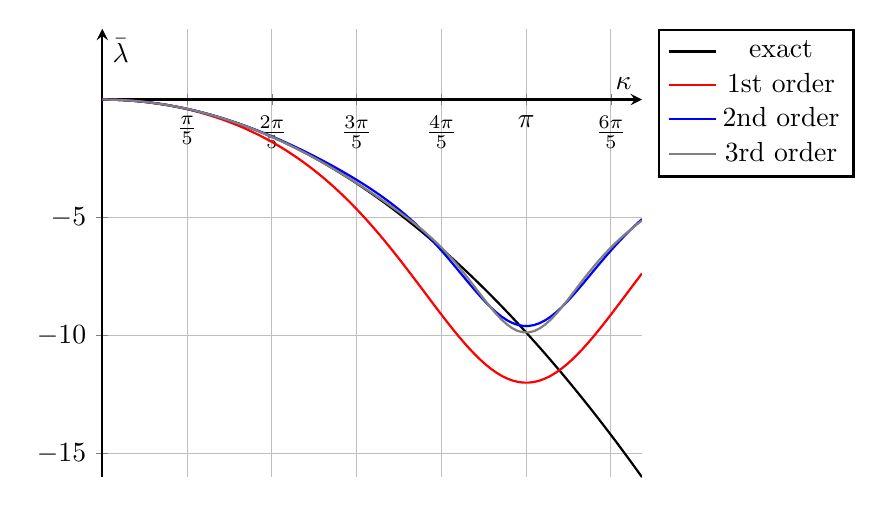
\begin{tikzpicture}
\begin{axis}[ xlabel={$\kappa$}, ylabel={$\bar{\lambda}$}
  ,axis x line=middle,axis y line=middle
  ,thick,grid,no marks,samples=101
  ,domain=0:4,ymax=3
  ,xtick={0.62832,1.25664,1.88496,2.51328,3.1416,3.76992}
  ,xticklabels={$\frac{\pi}{5}$,$\frac{2\pi}{5}$,$\frac{3\pi}{5}$,$\frac{4\pi}{5}$,$\pi$,$\frac{6\pi}{5}$}
  ,legend pos=outer north east
  ] 
\addplot[color=black]  {0-(x^2)}; 
\addlegendentry{exact};
\addplot[color=red] {-6*(1-cos(deg(x)))/(2+cos(deg(x)))}; 
\addlegendentry{1st order};
\addplot[color=blue] {-1/5*(96+27*cos(deg(x))-72*cos(deg(x))^2-51*cos(deg(x))^3)/(8+12*cos(deg(x))+6*cos(deg(x))^2+cos(deg(x))^3)}; 
\addlegendentry{2nd order};
\addplot[color=gray] {1/175*(-13824-17010*cos(deg(x))+4050*cos(deg(x))^2+15525*cos(deg(x))^3+8910*cos(deg(x))^4+2349*cos(deg(x))^5)
/(32+80*cos(deg(x))+80*cos(deg(x))^2+40*cos(deg(x))^3+10*cos(deg(x))^4+cos(deg(x))^5)
}; 
\addlegendentry{3rd order};
\end{axis}
\end{tikzpicture}
\caption{The  non-dimensionalised spectrum 
($\bar{\lambda}=\lambda H^2/\nu$ versus $\kappa=kH$)
of the diffusion equation
($\alpha=0$) for the mode $\tilde{u}(x,t)=e^{\lambda t+ik x}$, 
contrasting the continuum dynamics  against successive discrete, holistic approximations (for $\gamma=1$).}
\label{fig:diff:spectrum}
\end{figure}


\section{Numerical stability}\label{sec:numeric}
To investigate the theoretical stability of discrete approximations to Burgers' equation~\eqref{eq:burgers}, we
follow \cite{Foias} and consider a mostly undisturbed system where $U_j=0$ at all grid-points
except for $M$ adjacent, internal points. For example, for $M=2$ it suffices to choose $N=3$ with
$U_0=U_3=0$. Hence, with the transformation $U_j=\frac{\nu}{\alpha H}V_j$, 
the mixture model~\eqref{eq:mixture} reduces to
\begin{eqnarray}
\frac{H^2}{\nu}\dot{V}_1 & = & -2V_1+V_2-\frac{(1-\theta)}{2}V_1V_2-\frac{\theta}{4}V_2^2\,,
\\
\frac{H^2}{\nu}\dot{V}_2 & = & V_1-2V_2+\frac{(1-\theta)}{2}V_1V_2+\frac{\theta}{4}V_1^2\,.
\end{eqnarray}
This reduced system has a stable critical point at $V_1=V_2=0$ with non-dimensionalised eigenvalues 
$\bar{\lambda}=\frac{H^2}{\nu}\lambda=-1, -3$, and 
an unstable critical point at $V_1=-V_2=\frac{12}{2-3\theta}$
with eigenvalues $\bar{\lambda}=\frac{2}{2-3\theta}
\pm\frac{|4-9\theta|}{|2-3\theta|}$. 
Observe that the unstable point is removed to infinity when $\theta=\frac{2}{3}$.
This is exactly the critical value predicted by \cite{Fornberg73} to be necessary (but not always sufficient)
for numerical stability of the mixture model with $\nu=0, \alpha=1$.
Consequently, the corresponding reduction of the holistic model~\eqref{eq:holistic1}, namely
\begin{eqnarray}
\frac{H^2}{\nu}\dot{V}_1 & = & -4V_1+\frac{11}{4}V_2-\frac{1}{12}V_1^2-\frac{3}{8}V_1V_2-\frac{7}{24}V_2^2\,,
\\
\frac{H^2}{\nu}\dot{V}_2 & = & \frac{11}{4}V_1-4V_2+\frac{7}{24}V_1^2+\frac{3}{8}V_1V_2+\frac{1}{12}V_2^2\,,
\end{eqnarray}
is unconditionally stable with critical point at $V_1=V_2=0$ and eigenvalues $\bar{\lambda}= -\frac{5}{4}, -\frac{27}{4}$.

Similarly, for $M=3$ consecutive points the mixture model~\eqref{eq:mixture} reduces to
\begin{eqnarray}
\frac{H^2}{\nu}\dot{V}_1 & = & -2V_1+V_2-\frac{(1-\theta)}{2}V_1V_2-\frac{\theta}{4}V_2^2\,,
\\
\frac{H^2}{\nu}\dot{V}_2 & = & V_1-2V_2+V_3-\frac{(1-\theta)}{2}V_2(V_3-V_1)-\frac{\theta}{4}(V_3^2-V_1^2)\,,
\\
\frac{H^2}{\nu}\dot{V}_3 & = & V_2-2V_3+\frac{(1-\theta)}{2}V_2V_3+\frac{\theta}{4}V_2^2\,.
\end{eqnarray}
Substitution of $V_1=aV_2$ and $V_3=bV_2$ then leads to
\begin{eqnarray}
V_1=\frac{\mu(4-\mu\theta)}{8+2\mu(1-\theta)}\,, &
V_2=\mu\,, & V_3=\frac{\mu(4+\mu\theta)}{8-2\mu(1-\theta)}\,,
\end{eqnarray}
where $\mu$ satisfies
\begin{eqnarray}
\mu[\theta(1-\theta)(\theta^2-3\theta+1)\mu^4+16(2\theta^2-4\theta+1)\mu^2-256] = 0\,.
\end{eqnarray}
Observe that the coefficient of $\mu^4$ vanishes at $\theta=0, 1$ and $\theta_c=\frac{3-\sqrt{5}}{2}$.
It can then be shown that the trivial critical point (for $\mu=0$) is unconditionally stable, and that a pair of 
unstablel, nontrivial critical points occur when $0<\theta<\theta_c$.
Note that the holistic parameter value of $\theta=\frac{2}{3}$ lies in the range $\theta_c\le\theta\le 1$ for which there are no nontrivial critical points.

\section{Conclusion}


\bibliographystyle{agsm}
\IfFileExists{ajr.sty}
{\bibliography{bibexport,bib,ajr}}
{\bibliography{bibexport,yourbibfile}}


\end{document}
